\documentclass{vldb}
	\usepackage{balance}  % for  \balance command ON LAST PAGE  (only there!)	
	\usepackage {tikz}
	\usepackage{wrapfig}
		\usetikzlibrary {positioning}
		
		\usepackage[ruled,vlined,linesnumbered]{algorithm2e}
		\usepackage{pgfplots}
		\usepackage{adjustbox}
		\usepackage{multicol}
		\usepackage{caption}
		\usepackage{cite}
		\newcommand*{\rom}[1]{\expandafter\@slowromancap\romannumeral #1@}
		\usepackage{amsmath}
		\usepackage{amssymb}
		\usepackage{algpseudocode}
		\usepackage{algorithmicx}
		\usepackage{graphicx}
	%	\usepackage{caption}
		\usetikzlibrary{positioning}
		\definecolor {processblue}{cmyk}{0.96,0,0,0}
%\newtheorem{theorem}{Theorem}[section]		
%\newtheorem{lemma}[theorem]{Lemma}



\begin{document}
	\title{ Flexible Social Spatial Group Queries}
	
	\numberofauthors{2}
	
	\author{
	}
	
	\date{16 March 2017}
	\maketitle
	
	

	
	\begin{multicols}{2}
	\begin {figure}
			\begin{center}
			\scalebox{.5}{% GNUPLOT: LaTeX picture
\setlength{\unitlength}{0.240900pt}
\ifx\plotpoint\undefined\newsavebox{\plotpoint}\fi
\sbox{\plotpoint}{\rule[-0.200pt]{0.400pt}{0.400pt}}%
\begin{picture}(1500,900)(0,0)
\sbox{\plotpoint}{\rule[-0.200pt]{0.400pt}{0.400pt}}%
\put(431.0,183.0){\rule[-0.200pt]{4.818pt}{0.400pt}}
\put(411,183){\makebox(0,0)[r]{ 0}}
\put(1139.0,183.0){\rule[-0.200pt]{4.818pt}{0.400pt}}
\put(431.0,287.0){\rule[-0.200pt]{4.818pt}{0.400pt}}
\put(411,287){\makebox(0,0)[r]{ 10}}
\put(1139.0,287.0){\rule[-0.200pt]{4.818pt}{0.400pt}}
\put(431.0,391.0){\rule[-0.200pt]{4.818pt}{0.400pt}}
\put(411,391){\makebox(0,0)[r]{ 20}}
\put(1139.0,391.0){\rule[-0.200pt]{4.818pt}{0.400pt}}
\put(431.0,495.0){\rule[-0.200pt]{4.818pt}{0.400pt}}
\put(411,495){\makebox(0,0)[r]{ 30}}
\put(1139.0,495.0){\rule[-0.200pt]{4.818pt}{0.400pt}}
\put(431.0,599.0){\rule[-0.200pt]{4.818pt}{0.400pt}}
\put(411,599){\makebox(0,0)[r]{ 40}}
\put(1139.0,599.0){\rule[-0.200pt]{4.818pt}{0.400pt}}
\put(431.0,703.0){\rule[-0.200pt]{4.818pt}{0.400pt}}
\put(411,703){\makebox(0,0)[r]{ 50}}
\put(1139.0,703.0){\rule[-0.200pt]{4.818pt}{0.400pt}}
\put(431.0,807.0){\rule[-0.200pt]{4.818pt}{0.400pt}}
\put(411,807){\makebox(0,0)[r]{ 60}}
\put(1139.0,807.0){\rule[-0.200pt]{4.818pt}{0.400pt}}
\put(464.0,131.0){\rule[-0.200pt]{0.400pt}{4.818pt}}
\put(464,90){\makebox(0,0){ 4}}
\put(464.0,839.0){\rule[-0.200pt]{0.400pt}{4.818pt}}
\put(630.0,131.0){\rule[-0.200pt]{0.400pt}{4.818pt}}
\put(630,90){\makebox(0,0){ 5}}
\put(630.0,839.0){\rule[-0.200pt]{0.400pt}{4.818pt}}
\put(795.0,131.0){\rule[-0.200pt]{0.400pt}{4.818pt}}
\put(795,90){\makebox(0,0){ 6}}
\put(795.0,839.0){\rule[-0.200pt]{0.400pt}{4.818pt}}
\put(960.0,131.0){\rule[-0.200pt]{0.400pt}{4.818pt}}
\put(960,90){\makebox(0,0){ 7}}
\put(960.0,839.0){\rule[-0.200pt]{0.400pt}{4.818pt}}
\put(1126.0,131.0){\rule[-0.200pt]{0.400pt}{4.818pt}}
\put(1126,90){\makebox(0,0){ 8}}
\put(1126.0,839.0){\rule[-0.200pt]{0.400pt}{4.818pt}}
\put(431.0,131.0){\rule[-0.200pt]{0.400pt}{175.375pt}}
\put(431.0,131.0){\rule[-0.200pt]{175.375pt}{0.400pt}}
\put(1159.0,131.0){\rule[-0.200pt]{0.400pt}{175.375pt}}
\put(431.0,859.0){\rule[-0.200pt]{175.375pt}{0.400pt}}
\put(310,495){\makebox(0,0){\rotatebox{90}{node x $10^3$}}}
\put(795,29){\makebox(0,0){min group size $n'$}}
\put(999,819){\makebox(0,0)[r]{Baseline}}
\put(1019.0,819.0){\rule[-0.200pt]{24.090pt}{0.400pt}}
\put(464,201){\usebox{\plotpoint}}
\multiput(464.00,201.58)(1.941,0.498){83}{\rule{1.644pt}{0.120pt}}
\multiput(464.00,200.17)(162.587,43.000){2}{\rule{0.822pt}{0.400pt}}
\multiput(630.00,244.58)(0.794,0.499){205}{\rule{0.735pt}{0.120pt}}
\multiput(630.00,243.17)(163.475,104.000){2}{\rule{0.367pt}{0.400pt}}
\multiput(795.58,348.00)(0.500,0.582){327}{\rule{0.120pt}{0.565pt}}
\multiput(794.17,348.00)(165.000,190.826){2}{\rule{0.400pt}{0.283pt}}
\multiput(960.58,540.00)(0.500,0.811){329}{\rule{0.120pt}{0.748pt}}
\multiput(959.17,540.00)(166.000,267.447){2}{\rule{0.400pt}{0.374pt}}
\put(464,201){\makebox(0,0){$\bullet$}}
\put(630,244){\makebox(0,0){$\bullet$}}
\put(795,348){\makebox(0,0){$\bullet$}}
\put(960,540){\makebox(0,0){$\bullet$}}
\put(1126,809){\makebox(0,0){$\bullet$}}
\put(1069,819){\makebox(0,0){$\bullet$}}
\put(999,778){\makebox(0,0)[r]{SSTK}}
\put(1019.0,778.0){\rule[-0.200pt]{24.090pt}{0.400pt}}
\put(464,191){\usebox{\plotpoint}}
\multiput(464.00,191.58)(7.131,0.492){21}{\rule{5.633pt}{0.119pt}}
\multiput(464.00,190.17)(154.308,12.000){2}{\rule{2.817pt}{0.400pt}}
\multiput(630.00,203.58)(1.506,0.499){107}{\rule{1.300pt}{0.120pt}}
\multiput(630.00,202.17)(162.302,55.000){2}{\rule{0.650pt}{0.400pt}}
\multiput(795.00,258.58)(1.335,0.499){121}{\rule{1.165pt}{0.120pt}}
\multiput(795.00,257.17)(162.583,62.000){2}{\rule{0.582pt}{0.400pt}}
\multiput(960.00,320.58)(0.509,0.500){323}{\rule{0.507pt}{0.120pt}}
\multiput(960.00,319.17)(164.947,163.000){2}{\rule{0.254pt}{0.400pt}}
\put(464,191){\makebox(0,0){$\blacktriangle$}}
\put(630,203){\makebox(0,0){$\blacktriangle$}}
\put(795,258){\makebox(0,0){$\blacktriangle$}}
\put(960,320){\makebox(0,0){$\blacktriangle$}}
\put(1126,483){\makebox(0,0){$\blacktriangle$}}
\put(1069,778){\makebox(0,0){$\blacktriangle$}}
\put(999,737){\makebox(0,0)[r]{Approximate}}
\put(1019.0,737.0){\rule[-0.200pt]{24.090pt}{0.400pt}}
\put(464,184){\usebox{\plotpoint}}
\put(464,184.17){\rule{33.300pt}{0.400pt}}
\multiput(464.00,183.17)(96.884,2.000){2}{\rule{16.650pt}{0.400pt}}
\put(630,185.67){\rule{39.749pt}{0.400pt}}
\multiput(630.00,185.17)(82.500,1.000){2}{\rule{19.874pt}{0.400pt}}
\multiput(795.00,187.60)(24.023,0.468){5}{\rule{16.600pt}{0.113pt}}
\multiput(795.00,186.17)(130.546,4.000){2}{\rule{8.300pt}{0.400pt}}
\put(464,184){\makebox(0,0){$\blacksquare$}}
\put(630,186){\makebox(0,0){$\blacksquare$}}
\put(795,187){\makebox(0,0){$\blacksquare$}}
\put(960,191){\makebox(0,0){$\blacksquare$}}
\put(1126,191){\makebox(0,0){$\blacksquare$}}
\put(1069,737){\makebox(0,0){$\blacksquare$}}
\put(960.0,191.0){\rule[-0.200pt]{39.989pt}{0.400pt}}
\put(431.0,131.0){\rule[-0.200pt]{0.400pt}{175.375pt}}
\put(431.0,131.0){\rule[-0.200pt]{175.375pt}{0.400pt}}
\put(1159.0,131.0){\rule[-0.200pt]{0.400pt}{175.375pt}}
\put(431.0,859.0){\rule[-0.200pt]{175.375pt}{0.400pt}}
\end{picture}
}
			\end{center}
			\caption{ small dataset $( c=2, d_m=10) $}
			\end {figure}
		    
	
	\begin {figure}
			\begin{center}
			\scalebox{.5}{% GNUPLOT: LaTeX picture
\setlength{\unitlength}{0.240900pt}
\ifx\plotpoint\undefined\newsavebox{\plotpoint}\fi
\sbox{\plotpoint}{\rule[-0.200pt]{0.400pt}{0.400pt}}%
\begin{picture}(1500,900)(0,0)
\sbox{\plotpoint}{\rule[-0.200pt]{0.400pt}{0.400pt}}%
\put(431.0,183.0){\rule[-0.200pt]{4.818pt}{0.400pt}}
\put(411,183){\makebox(0,0)[r]{ 0}}
\put(1139.0,183.0){\rule[-0.200pt]{4.818pt}{0.400pt}}
\put(431.0,287.0){\rule[-0.200pt]{4.818pt}{0.400pt}}
\put(411,287){\makebox(0,0)[r]{ 10}}
\put(1139.0,287.0){\rule[-0.200pt]{4.818pt}{0.400pt}}
\put(431.0,391.0){\rule[-0.200pt]{4.818pt}{0.400pt}}
\put(411,391){\makebox(0,0)[r]{ 20}}
\put(1139.0,391.0){\rule[-0.200pt]{4.818pt}{0.400pt}}
\put(431.0,495.0){\rule[-0.200pt]{4.818pt}{0.400pt}}
\put(411,495){\makebox(0,0)[r]{ 30}}
\put(1139.0,495.0){\rule[-0.200pt]{4.818pt}{0.400pt}}
\put(431.0,599.0){\rule[-0.200pt]{4.818pt}{0.400pt}}
\put(411,599){\makebox(0,0)[r]{ 40}}
\put(1139.0,599.0){\rule[-0.200pt]{4.818pt}{0.400pt}}
\put(431.0,703.0){\rule[-0.200pt]{4.818pt}{0.400pt}}
\put(411,703){\makebox(0,0)[r]{ 50}}
\put(1139.0,703.0){\rule[-0.200pt]{4.818pt}{0.400pt}}
\put(431.0,807.0){\rule[-0.200pt]{4.818pt}{0.400pt}}
\put(411,807){\makebox(0,0)[r]{ 60}}
\put(1139.0,807.0){\rule[-0.200pt]{4.818pt}{0.400pt}}
\put(464.0,131.0){\rule[-0.200pt]{0.400pt}{4.818pt}}
\put(464,90){\makebox(0,0){ 4}}
\put(464.0,839.0){\rule[-0.200pt]{0.400pt}{4.818pt}}
\put(630.0,131.0){\rule[-0.200pt]{0.400pt}{4.818pt}}
\put(630,90){\makebox(0,0){ 5}}
\put(630.0,839.0){\rule[-0.200pt]{0.400pt}{4.818pt}}
\put(795.0,131.0){\rule[-0.200pt]{0.400pt}{4.818pt}}
\put(795,90){\makebox(0,0){ 6}}
\put(795.0,839.0){\rule[-0.200pt]{0.400pt}{4.818pt}}
\put(960.0,131.0){\rule[-0.200pt]{0.400pt}{4.818pt}}
\put(960,90){\makebox(0,0){ 7}}
\put(960.0,839.0){\rule[-0.200pt]{0.400pt}{4.818pt}}
\put(1126.0,131.0){\rule[-0.200pt]{0.400pt}{4.818pt}}
\put(1126,90){\makebox(0,0){ 8}}
\put(1126.0,839.0){\rule[-0.200pt]{0.400pt}{4.818pt}}
\put(431.0,131.0){\rule[-0.200pt]{0.400pt}{175.375pt}}
\put(431.0,131.0){\rule[-0.200pt]{175.375pt}{0.400pt}}
\put(1159.0,131.0){\rule[-0.200pt]{0.400pt}{175.375pt}}
\put(431.0,859.0){\rule[-0.200pt]{175.375pt}{0.400pt}}
\put(310,495){\makebox(0,0){\rotatebox{90}{node x $10^3$}}}
\put(795,29){\makebox(0,0){min group size $n'$}}
\put(999,819){\makebox(0,0)[r]{Baseline}}
\put(1019.0,819.0){\rule[-0.200pt]{24.090pt}{0.400pt}}
\put(464,201){\usebox{\plotpoint}}
\multiput(464.00,201.58)(1.941,0.498){83}{\rule{1.644pt}{0.120pt}}
\multiput(464.00,200.17)(162.587,43.000){2}{\rule{0.822pt}{0.400pt}}
\multiput(630.00,244.58)(0.794,0.499){205}{\rule{0.735pt}{0.120pt}}
\multiput(630.00,243.17)(163.475,104.000){2}{\rule{0.367pt}{0.400pt}}
\multiput(795.58,348.00)(0.500,0.582){327}{\rule{0.120pt}{0.565pt}}
\multiput(794.17,348.00)(165.000,190.826){2}{\rule{0.400pt}{0.283pt}}
\multiput(960.58,540.00)(0.500,0.811){329}{\rule{0.120pt}{0.748pt}}
\multiput(959.17,540.00)(166.000,267.447){2}{\rule{0.400pt}{0.374pt}}
\put(464,201){\makebox(0,0){$\bullet$}}
\put(630,244){\makebox(0,0){$\bullet$}}
\put(795,348){\makebox(0,0){$\bullet$}}
\put(960,540){\makebox(0,0){$\bullet$}}
\put(1126,809){\makebox(0,0){$\bullet$}}
\put(1069,819){\makebox(0,0){$\bullet$}}
\put(999,778){\makebox(0,0)[r]{SSTK}}
\put(1019.0,778.0){\rule[-0.200pt]{24.090pt}{0.400pt}}
\put(464,191){\usebox{\plotpoint}}
\multiput(464.00,191.58)(7.131,0.492){21}{\rule{5.633pt}{0.119pt}}
\multiput(464.00,190.17)(154.308,12.000){2}{\rule{2.817pt}{0.400pt}}
\multiput(630.00,203.58)(1.506,0.499){107}{\rule{1.300pt}{0.120pt}}
\multiput(630.00,202.17)(162.302,55.000){2}{\rule{0.650pt}{0.400pt}}
\multiput(795.00,258.58)(1.335,0.499){121}{\rule{1.165pt}{0.120pt}}
\multiput(795.00,257.17)(162.583,62.000){2}{\rule{0.582pt}{0.400pt}}
\multiput(960.00,320.58)(0.509,0.500){323}{\rule{0.507pt}{0.120pt}}
\multiput(960.00,319.17)(164.947,163.000){2}{\rule{0.254pt}{0.400pt}}
\put(464,191){\makebox(0,0){$\blacktriangle$}}
\put(630,203){\makebox(0,0){$\blacktriangle$}}
\put(795,258){\makebox(0,0){$\blacktriangle$}}
\put(960,320){\makebox(0,0){$\blacktriangle$}}
\put(1126,483){\makebox(0,0){$\blacktriangle$}}
\put(1069,778){\makebox(0,0){$\blacktriangle$}}
\put(999,737){\makebox(0,0)[r]{Approximate}}
\put(1019.0,737.0){\rule[-0.200pt]{24.090pt}{0.400pt}}
\put(464,184){\usebox{\plotpoint}}
\put(464,184.17){\rule{33.300pt}{0.400pt}}
\multiput(464.00,183.17)(96.884,2.000){2}{\rule{16.650pt}{0.400pt}}
\put(630,185.67){\rule{39.749pt}{0.400pt}}
\multiput(630.00,185.17)(82.500,1.000){2}{\rule{19.874pt}{0.400pt}}
\multiput(795.00,187.60)(24.023,0.468){5}{\rule{16.600pt}{0.113pt}}
\multiput(795.00,186.17)(130.546,4.000){2}{\rule{8.300pt}{0.400pt}}
\put(464,184){\makebox(0,0){$\blacksquare$}}
\put(630,186){\makebox(0,0){$\blacksquare$}}
\put(795,187){\makebox(0,0){$\blacksquare$}}
\put(960,191){\makebox(0,0){$\blacksquare$}}
\put(1126,191){\makebox(0,0){$\blacksquare$}}
\put(1069,737){\makebox(0,0){$\blacksquare$}}
\put(960.0,191.0){\rule[-0.200pt]{39.989pt}{0.400pt}}
\put(431.0,131.0){\rule[-0.200pt]{0.400pt}{175.375pt}}
\put(431.0,131.0){\rule[-0.200pt]{175.375pt}{0.400pt}}
\put(1159.0,131.0){\rule[-0.200pt]{0.400pt}{175.375pt}}
\put(431.0,859.0){\rule[-0.200pt]{175.375pt}{0.400pt}}
\end{picture}
}
			\end{center}
			\caption{ small dataset $( c=2, d_m=10) $}
	\end {figure}
		
	
	
	\end{multicols}
	


















	\section{Introduction}
		Social connectivity over social network helps forming groups outside physical world. Location based service through smartphone and other networks helps tracking a person's activity. Now socio spatial group queries are considered where the main purpose is to find a group of  people who are socially connected and are nearby to each others. There are various application of socio spatial group queries. Suppose a shop owner is interested in finding such a group for advertisement (e.g. Groupon )  or an user may want to find a group of friends to watch cinema at weekend.  Socio-spatial group queries for impromptu activity planning have been proposed \cite{shen2016socio}  that considers both social and spatial factors while finding a meet-up location for a fixed size group of nearby people with strong social connections. But fixed size group limits the applicability of socio-spatial queries. Without prior knowledge of the social graphs and user locations, it might be difficult for an advertiser to offer the best deal to users and at the same time maximize their profit. Thus the advertiser may want to know different size of subgroups with various social and spatial constraints. For example, there is a traditional "buy two get one" offer. But advertiser might have found out that, most of the groups are generally of 4 people. So 3 member size group does not come out as a feasible offer. 
		
		
		
		
		Increasing group size may increase profit of advertiser. But increasing the group size may decrease a user's social satisfaction in the meet-up as it increases the chance of meeting more unknown people. Thus we can see that there is trade off between satisfaction and cost in such queries and finding the optimal group size is essential for such scenarios.  Zhu et al.  \cite{zhu2014geo} proposed a new class of geo-social group queries with minimum acquaintance constraint (GSGQs), where the identified group guarantees the worst-case acquaintance level of all users. We incorporate the idea of minimum acquaintance constraint in our problem so that members in a group satisfy that every individual is acquainted with at least a minimum number of other members in that group. \cite{zhu2014geo} 
		targets at finding a group where query issuer is  an user . Here an user targets at finding a group having strong social connectivity satisfying worst level acquaintance and minimized 
		spatial distance from query issuer. So in the resultant group, that particular user must be included which limits applicability of socio spatial group queries as it only satisfies the situation where an user is planning to have a weekend party with friends and friends of friends. But an advertiser , if interested to provide coupon to a group of people, doesn't necessarily needs to be socially connected with people of that group. \cite{yang2012socio}  finds out a group against one rally point whereas \cite{shen2016socio} considers multiple rally points. Both target at finding the best group which doesn't necessarily meet up applicability of  socio spatial group queries since finding one group from a huge socio spatial graph is not worth mentioning. So we aim at -
		\begin{itemize}
		\item finding group ensuring that member of any group satisfies minimum acquaintance constraint within the group.
		
		\item considering group having relaxed group size greater than a minimum value.
		
		\item developing a ranking function focused on strong social connectivity, minimized spatial distance and group size.
								
		\item finding top $ k $ groups against multiple points of interest ( POI) which denotes the locations of meeting point or locations of business owners.
		
		\end{itemize}
		
		\section{Problem Formulation :} Given a social graph $ G = (V, E) $, location of each user $ l_v , v \in V$ , minimum acquaintance constraint c, minimum number of users $ n' $ in the resulting group , the set of candidate meeting
		points $ O $. We will find top $ k $ best groups (each group with minimum $ n' $ users ) and the
		corresponding meeting points $ o' $ in order of their socio social ranking.
		
		
		
		To rank the groups Socio spatial ranking function SSRF will prioritize the following attributes of those groups.
		
		\begin{enumerate}
		\item \textbf{Spatial distance:} The resulting group ensures that total spatial distance from target meeting point $ o' $ is minimized.
		\item \textbf{Social Connectivity:} A more social connected group is desirable. So the rank function will consider social connectivity in the following ways.
			\begin{itemize}
			\item \textbf{Minimum acquaintance:}  A group must ensure that every member in that group has connectivity greater than a minimum constraint $ c $.
			\item \textbf{Average Connectivity:} When two groups satisfy minimum constraint, the group having more average social connectivity should be ranked higher.	
			\end{itemize}
		\item \textbf{Group size:} Our  goal is to find groups having  members $ \geq n' $ provided that social connectivity is maximized and spatial distance is minimized. 
		\end{enumerate}
		
		\section{Objective Function :} Let $ G'=(V',E'),G' \in G $ be a derived graph (resulting group) , $ c $ be minimum acquaintance constraint , $ n' $ be  minimum number of users in $ G' $ and $o' \in  O $ is target meeting point for $ V' $. Here  $ V' $ is the set of members of that group and $ uv \in E', u,v \in V' $ means member u and v are acquainted with each other. Our objective is to take care of the following issues-
		\begin{itemize}
		\item[] (\romannumeral 1)  $\forall v_i \in V', f(v_i,V') \geq c  $. $ f(v_i,V')$ returns number of members in group $ V' $ with whom $ v_i $ is acquainted with.
		
		\item[] (\romannumeral 2)   $ \bar{f}(V') $ which returns the average social connectivity of a group provided that  (\romannumeral 1) is satisfied.
		\item[] (\romannumeral 3)  group size of $ V' $, $ |V'| \geq n' $.
		\item[] (\romannumeral 4)   average spatial distance $  \frac{1}{|V'|} \sum_{v_i \in V'} d(v_i,o') $. Here $ d(v_i,o') $ gives spatial distance between member $ v_i $ and target meeting point $ o' $.
		
		\end{itemize}   
		Here (\romannumeral 2) represents social aspect, (\romannumeral 4) represents spatial aspect and (\romannumeral 3) emphasis on size of group.  Higher value of  (\romannumeral 2) and (\romannumeral 3) and lower value of (\romannumeral 4) will result in higher score by SSRF.
		
		
		
		 
		
		
		\begin{figure}[t]
				\centerline{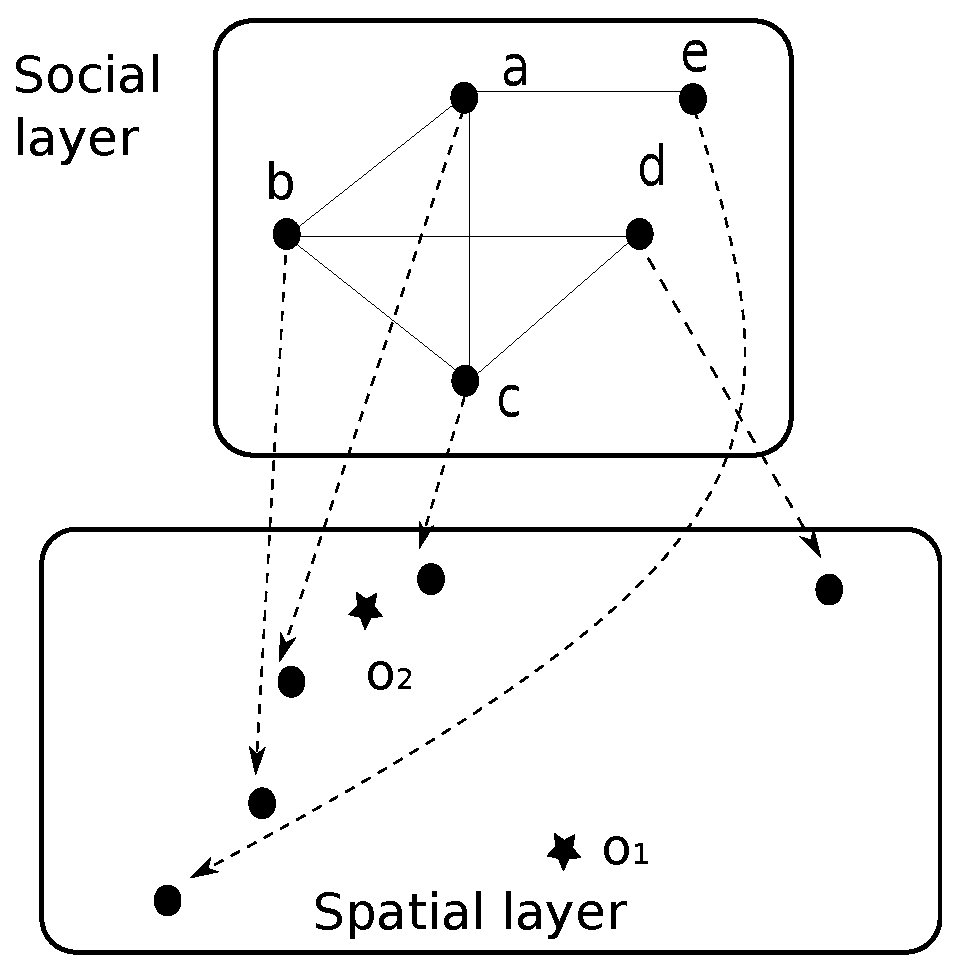
\includegraphics[width=.4\columnwidth]{drawing2}}
				\caption{Socio spatial graph}
				\label{fig:graph1}
		\end{figure}
		
		
		
		\subsection*{Motivating Example} Figure:~\ref{fig:graph1} represents a socio-spatial graph where the upper rectangle represents social layer and lower rectangle represents spatial layer. Here $ V=\{a,b,c,d,e\} $ represents set of members in given graph where every edge in social layer represents social connectivity between two individuals.  An arrow from each member in social layer represents corresponding location in spatial layer.   $ O=\{o_{1},o_{2}\} $ is location set of meeting points in spatial layer. Suppose we are interested in finding out top-$ k $ groups with members not less than 3. The resulting group satisfies minimum acquaintance constraint $ c=1 $. For meeting point $ o_{1} $ existing paper \cite{yang2012socio} would find a group of $ \{a,b,e\} $ where each member is acquainted with at least one other member in resulting group, thus satisfying minimum acquaintance constraint. Let's assume our ranking function gives score 6 out of 10 to group $ \{a,b,e\} $. But we will show that adding $ d $ in resulting group would give a better score (i.e. 7 out of 10 ) than the previous one according to socio-spatial ranking function and this new group also satisfies all required conditions. If group size was strictly maintained, potential members would have been deprived in spite of having better social connectivity and spatial location. Here average social connectivity has decreased and total spatial distance has increased but increase in group size has surpassed both .
		
		
		
		
		
		
		\section{Socio Spatial Ranking Function SSRF:}
		Now we will provide formal definition of SSRF. SSRF takes $ 4 $ parameter as input- graph $ G'=(V',E'),G' \in G $, target meeting point $ o' $,  minimum group size $ n' $ and minimum acquaintance constraint $ c $. SSRF can be represented as $ R(G',o',n',c) $. 
		SSRF returns a score value for $ G' $. This score can be subdivided into three category- social connectivity , spatial position and group size.   
		\subsection{Social connectivity score: } 
		To measure social score of group $ G' $, we need to calculate  $ f(v,V')$  and  $\bar{f}(V') $. For two members $ u $ and $ v ,u,v \in V'$, we can define a function $ \hat{f}(u,v) $ in the following way.
		\begin{equation*}
		\hat{f}(u,v)=
		\begin{cases}
		\text{1,} & \quad\text{$ uv \in E' $}\\
		\text{0} & \quad\text{otherwise}							
		\end{cases}
		\end{equation*}
		
		Now $ f(v,V'),v \in V'$ can be easily calculated.
		
		\[
		f(v,V')=\sum_{u \in V', v\neq u} \hat{f}(u,v)
		\]
		
		
		$ f(v,V')$ is  within  [0,$ |V'|-1 $ ]. So $\bar{f}(V') $ can be derived in the following way.
		
		
		\[
		\bar{f}(V')=\frac{1}{|V'|} \sum_{v_i \in V'} f(v_i,V')
		\]
		
		
		Social connectivity score, $ S_{sc} $ is normalized form of   $ \bar{f}(V') $ and within [0,1] range.
		
		\begin{equation*}
			S_{sc}=
			\begin{cases}
			\text{$ \frac{\bar{f}(V')}{|V'|-1} $,} & \quad\text{$ 	\forall v_i\in V',f(v_i,V') \geq c $}\\
			\text{0} & \quad\text{otherwise}							
			\end{cases}
		\end{equation*}
		
		Here, we must ensure that every member in the group must satisfy minimum acquaintance constraint.
	
		
		
		
		\subsection{Spatial position score:} 
		A group will be ahead in ranking if its spatial distance is minimized. So spatial score is inversely related with spatial distance.  For given graph $ G' $ and  meeting point $ o' $  spatial
		position score, $ S_{sp} $ can be defined in the following way-
		
		\[
		S_{sp}=1- \frac{\sum_{v_i \in V'} d(v_i,o')}{d_{m}*|V'|} 
		\]
		
		$ S_{sp} $ will be within [0,1] range. Here $ d_{m} $ is a given parameter which bounds our search. We safely assume that no group will be generated where any member's location from meeting point is more than $ d_{m} $. 
		
		\[
		\forall v_i \in V', d(v_i,o')<=d_{m}
		\]
		
		
		
		\subsection{Group size score:}
		A group $ G' $ having members not less than $ n' $ is scored based on it's number of members. SO group size score $S_{gs} $ is computed in the following way- 
		
		\[
			S_{gs}=
				\begin{cases}
				\text{$ \frac{|V'|}{|V|} $,} & \quad\text{$ |V'|\geq n'$}\\
				\text{0} & \quad\text{otherwise}							
				\end{cases}
		\]
		
		\subsection{Group score:} 
		We have shown how to calculate  social ,spatial  and group size score of a particular group. All these scores are normalized. So the final ranking function will be a combination of social score, spatial score and group size score. 
		
		
		
		\begin{equation}
		\label{eq:score}
		S=\alpha*S_{sc} + \beta*S_{sp} + \gamma*S_{gs} 
		\end{equation}  
		
		The value of $ \alpha, \beta $ and $ \gamma  $ can be defined based on priority over those factors. For simplicity, we may assume $ \alpha+ \beta+\gamma = 1 $.
		
		
		
		
		\section{Socio spatial top  k  group query  SSGK:}
			Now we will formally define socio spatial top $ k $ group query SSGk. SSGk takes 4 parameters-  socio spatial graph $ G=(V,E) $,  minimum group size $ n' $,  minimum acquaintance constraint $ c $, number of groups to be ranked $ k $. SSGk returns a list $ L $ of $ k $ tuples where each tuple consists of a group $ G' $, score computed through SSRF and corresponding meeting point of $ G' $.		So SSGk can be represented as $ F(G,n',c,k) $ and the 
			resultant list $ L=\{(G_1,R(G_1,o_1,n',c),o_1),$ 
			\\ $ (G_2,R(G_2,o_2,n',c),o_2),  ....,	
			(G_k,R(G_k,o_k,n',c),o_k)\} $ . This list is prepared in descending order of score through SSRF and any other tuple not included in this list must have lower score than any group in $ L $. So  for $ 1\leq i\leq k $-

			
			\begin{align*}
			\begin{split}
			R(G_i,o_i,n',c) \geq R(G_{i+1},o_{i+1},n',c) \wedge 
			\\
			(\nexists (G_l,R(G_l,o_l,n',c),o_l)
			\notin R:
			\\
			R(G_K,o_k,n',c) \leq R(G_l,o_l,n',c) )
			\end{split}
			\end{align*}
			
			
			
			
			
			
		
		
		\section{Baseline Algorithm:}
		Our baseline algorithm is quite straight-forward. For each meeting point $ o_i, o_i \in O $, we will consider two set of members, $ V_I $ and $ V_R $. Initially $ V_I=\varnothing $ and $ V_R $ contains those members who are within a circular area of radius $ d_m $. Members are indexed by R-tree structure and included in $ V_R $ in ascending order of distance from $ o_i $. 
		Then we call $ findGroup $ function for current $ V_I, V_R $ and $ o_i $. At each iteration we retrieve member $ v $ from $ V_R $ which is least distant from $ o_i $ for current $ o_i $. We include $ v $ in $ V_I $ and call $ findGroup $ for updated $ V_I$ and $ V_R $. Our primary target is to find a group of minimum $ n' $ members. So when  $ V_I=n' $, we check whether $ V_I $ satisfies minimum acquaintance constraint, i.e. each member in $ V_I $ is familiar with at least $ c $ other members in $ V_I $. If current $ V_I $ satisfies this condition we update result list for currently found group. We further proceed for other members as we are willing in finding group for more than $ n' $ members. Our search finishes until there is any unvisited member left in $ V_R $. If $ V_I $ fails to satisfy familiarity constraint, we backtrack and remove last included member from $ V_I $ and search of rest of the members in $ V_R $. This baseline algorithm generates each possible combination of search space which is quite inefficient . So in the later section we are proposing some heuristic approach and pruning condition to avoid unnecessary searching and thus reducing running time. 
		
		\section{Our Approach:}
		The baseline algorithm performs badly as initially it includes members from $ V_R $ to $ V_I $ without proper judgment. Most of the time the lest distant members are not necessarily socially connected. Again, situation might arise where members in $ V_R $ are not even connected with at least $ c $ other members in $ V_R $. So these members can't satisfy familiarity constraint since the resultant group would be a subset of $ V_R $. So in our approach we first remove those members who fail to satisfy familiarity constraint even in $ V_R $. 
		
		The modified $ V_R $ is more probable to result in satisfactory group. Now while choosing initial members for $ V_I $ , the following equation will decide whether $ v $ to be considered to be included in $ V_I $. 
		
		\begin{equation}
			\label{eq:familiarityLowerBound}
			f(v,V_I)>= \bigg\lfloor\frac{c*|V_I|}{n'-1}\bigg\rfloor
		\end{equation}
		
		In Eq. ~\ref{eq:familiarityLowerBound}, $ f(v,V_I) $ denotes number of friends of member $ v $ in $ V_I $ and  member $ v $ is retrieved from $ V_R $ to be possibly included in $ V_I $. In our problem formulation each member in minimum $ n' $ sized group must know at least $ c $ members from other $ n'-1 $ members. So according to unitary method member $ v $, if considered to be included in $ V_I $ must satisfy the above condition. Let's assume, $ n'=5, $  $ c=2 $ and $ |V_I|=1 $ . So $ v $ must have to be acquainted with at least $ \lfloor\frac{2}{5-1} \rfloor=\lfloor\frac{1}{2} \rfloor = 0$ member . If floor part is omitted, then $ \frac{c*|V_I|}{n'-1} $ would be turned to $ \big\lceil\frac{c*|V_I|}{n'-1}\big\rceil $ since, $ f(v,V_I) $ returns an integer value. 
		
		\begin{equation}
			\label{eq:familiarityUpperBound}
			f(v,V_I)>=\frac{c*|V_I|}{n'-1}= \bigg\lceil\frac{c*|V_I|}{n'-1}\bigg\rceil
		\end{equation}

		Eq. ~\ref{eq:familiarityUpperBound}		provides a tighter bound of social connection on $ v $. Both Eq. ~\ref{eq:familiarityLowerBound} and ~\ref{eq:familiarityUpperBound} don't guarantee $ V_I $ to be  a group where each member satisfies minimum acquaintance constraint. But the resulting group which satisfies  Eq. ~\ref{eq:familiarityUpperBound} maintains average social connectivity greater or equal than minimum acquaintance level. 
		At each iteration when a new member is considered to be included in $ V_I $, $ V_I $ is multiplied by a factor of $ \frac{c}{n'-1} $. Initially $ |V_I|=0 $ and for the last member to be considered inclusion in a group of $ n' $ size, $ |V_I|=n'-1 $.
		
		\begin{equation*}
		\begin{aligned}
		\begin{split}
			&\frac{c}{n'-1}*0+\frac{c}{n'-1}*1+......+\frac{c}{n'-1}*(n'-1)\\
			&= \frac{c}{n'-1}*(0+1+2+.....+(n'-1))\\
			&= \frac{c}{n'-1}*\frac{(n'-1)*n'}{2}\\
			&= \frac{c*n'}{2}
						\end{split}
		\end{aligned}
		\end{equation*}
		
		Since when a member is socially connected with another member, social connectivity in the overall graph is increased by $ 2 $, so multiplying $ \frac{c*n'}{2} $ by $ 2 $ gives a total social connectivity of $ c*n' $ which satisfies the fact that resulting group of $ n' $ size maintains a minimum total social connectivity of $ c*n' $, i.e. minimum average social connectivity of $ c $ which is  minimum acquaintance constraint. But as we are more interested for each member to satisfy minimum acquaintance constraint, before considering $ V_I $ as possible resultant group, we must check the min degree of $ V_I $, $ \delta(V_I) $ according to following equation.
		\begin{equation}
			\delta(V_I)>=c
		\end{equation}
		
		If the above condition does not hold, we need to backtrack and try to find out other feasible solution. 
		It is obvious that some members are not included if Eq. ~\ref{eq:familiarityLowerBound} or ~\ref{eq:familiarityUpperBound}  is counted while including members in $ V_I $. So we will proof by contradiction that if any member $ v $ fails to satisfy ~\ref{eq:familiarityLowerBound} or ~\ref{eq:familiarityUpperBound}, resulting group including $ v $ would never result in a feasible group. 
		%f(v,V_I)>= \bigg\lfloor\frac{c*|V_I|}{n'-1}\bigg\rfloor
		\newtheorem{Lemma}{Lemma}
		\begin{Lemma}
		For any member $ v, v \notin V_I $, if $ f(v,V_I)< \big\lfloor\frac{c*|V_I|}{n'-1}\big\rfloor $, $ v $ can be considered not included in $ V_I $ and it will not exclude any feasible resultant group.
		\end{Lemma}
		
		\begin{proof}
		Let's assume, already $ n'-1 $ members are included in $ V_I $. From R-tree indexing, member $ v $ is extracted from $ V_R $. Now R.H.S of Eq. ~\eqref{eq:familiarityLowerBound} is $ \big\lfloor\frac{c*|V_I|}{n'-1}\big\rfloor=\big\lfloor\frac{c*(n'-1)}{n'-1}\big\rfloor = c$.  Now if $ f(v,V_I)< c $, then resulting group $ V_I\cup\{v\} $ will not satisfy familiarity constraint as  $ |V_I\cup\{v\}|=n' $ and min degree of $ V_I\cup\{v\} $ , $ \delta(V_I\cup\{v\})<c $. This proof is easy when we assume $ |V_I|=n-1 $. Now in general we assume $ |V_I|=\frac{k*(n'-1)}{c} $ where $ k  $ is any arbitrary integer and $ 0<=k<=c $. Now $ \big\lfloor\frac{c*}{n'-1}*\frac{k*(n'-1)}{c}\big\rfloor =\big\lfloor k\big\rfloor=k$ and $ f(v,V_I)< k $ which means $ f(v,V_I)=k-1 $ in the best case . Now in $ |V_I|=\frac{k*(n'-1)}{c} $ members , $ v $ is familiar with $ k-1 $ members  in the best case. So at an average $ v $ is acquainted with $ (k-1)/\frac{k*(n'-1)}{c} =\frac{k-1}{k}*\frac{c}{n'-1}$ members. Still $ (n'-1)-|V_I| =(n'-1)-\frac{k*(n'-1)}{c}=(n'-1)*\frac{c-k}{c}$ members are to be included in $ V_I $ and to satisfy familiarity constraint $ v $ has to be acquainted with additional $ c-(k-1)=c-k+1 $ members among the next  $ (n'-1)*\frac{c-k}{c}  $ members. So at an average $ v $ will have to be acquainted with $ (c-k+1)/\big((n'-1)*\frac{c-k}{c}\big) =\frac{c-k+1}{c-k}*\frac{c}{n'-1}$. Here we have found that $ \frac{k-1}{k}*\frac{c}{n'-1} < \frac{c-k+1}{c-k}*\frac{c}{n'-1}$ as 
		\begin{equation*}
		\begin{aligned}
		\begin{split}
		&\bigg(\frac{k-1}{k}*\frac{c}{n'-1}\bigg) / \bigg(\frac{c-k+1}{c-k}*\frac{c}{n'-1} \bigg)		\\
		&= \frac{k-1}{k}*\frac{c-k}{c-k+1}<1
		\end{split}
		\end{aligned}
		\end{equation*}
		
		So member $ v $ has to be acquainted with more members in proportion with his acquaintance at current situation which is less probable. So we can safely not consider $ v $. As our algorithm backtracks , member $ v $ might be considered in future iteration.  
		\end{proof}
		
		Eq. ~\eqref{eq:familiarityUpperBound} wrongly exclude some potential members, so resulting group using Eq. ~\eqref{eq:familiarityUpperBound} gives approximate solution whose percentage of acceptance is shown in experimental section. 
		
		
		 
		\subsection{Terminating Conditions}	
		
		The baseline algorithm is inefficient as it searches until $ V_R $ is empty. Here we will propose some pruning strategy so that we can terminate before checking every member in $ V_R $.  
		We will continue including member in $ V_I $ until $ |V_I|=n' $. But in our problem we have relaxed $ |V_I| $ and we will continue exploring if we are guaranteed to get better groups and associated meeting point. If we continue including one more member in $ V_I $ the resulting group must provide better score than the present best. Let $ f_{c} $ and $ f_{n} $ be current total number of friends of all members in $ V_I $ and increased number of friends if additional one member is  included into $  V_I $. Then change in social connectivity score will be-
		\begin{equation*}
		\begin{split}
		\begin{aligned}
			\Delta   S_{sc}&=\frac{f_{c}+f_{n}}{(|V_I|+1)*|V_I|}-\frac{f_{c}}{|V_I|*(|V_I|-1)}
			\\
			&=\frac{f_c}{|V_I|}*\frac{(|V_I|-1)-(|V_I|+1)}{(|V_I|-1)*(|V_I|+1)}+\frac{f_n}{|V_I|*(|V_I|+1)}
			\\
			&=\frac{f_n}{|V_I|*(|V_I|+1)}-\frac{2f_c}{(|V_I|-1)*|V_I|*(|V_I|+1)}
			\\
			\Delta S_{sc}&=\frac{1}{|V_I|*(|V_I|+1)}\bigg(f_n-\frac{2f_c}{(|V_I|-1)}
			\bigg)
			\end{aligned}	
		\end{split}
		\end{equation*}
		
		
		For including one more member, group size will increase by one. So total change in group size score will be-
		\[
		\Delta S_{gs} = \frac{(|V'|+1)-|V'|}{|V|}=\frac{1}{|V|}
		\] 
		Now if $ d_c $ is current total spatial distance from meeting point to all members in $ V_I $ and $ d_{e} $ is the increased distance between newly included members and meeting point $ o' $ , then change in spatial score will be-
		\[
		\begin{split}
		\begin{aligned}
			\Delta S_{sp}&=\frac{d_{c}}{d_{m}*|V_I|}-\frac{d_{c}+d_{e}}{d_{m}*(|V_I|+1)}
		\\
		&=\frac{d_c}{d_m*|V_I|}-\frac{d_c}{d_m*(|V_I|+1)}-\frac{d_e}{d_m*(|V_I|+1)}
		\\
		&= \frac{d_c}{d_m*|V_I|*(|V_I|+1)}-\frac{d_e}{d_m*(|V_I|+1)}
		\\
		\Delta S_{sp}&=\frac{1}{d_m*(|V_I|+1)}\bigg(\frac{d_c}{|V_I|}-d_e\bigg)
		\end{aligned}
		\end{split}
	 	\]
		
		\[
		d_{c}= \sum_{v_i \in V_I} {d(v_i,o')}
		\]
		
		Our goal is to increase score $ S $ of the new group. So the new group must ensure that overall score for group size of $ (|V_I|+1) $ is greater than of size $ |V_I| $. 
		\begin{equation}
		\begin{split}
		\label{eq:better}
		\alpha*\Delta S_{sc} + \beta*\Delta S_{sp} + \gamma*\Delta S_{gs} > 0
		\end{split}		
		\end{equation}
			
		\begin{equation}
		\label{eq:targetEqn}
		\begin{split}
		\Rightarrow	
			\frac{\alpha}{|V_I|*(|V_I|+1)}\bigg(f_n-\frac{2f_c}{(|V_I|-1)}
					\bigg)+
			\\
			 \frac{\gamma}{|V|}+
			\frac{\beta}{d_m*(|V_I|+1)}\bigg(\frac{d_c}{|V_I|}-d_e\bigg) > 0
		\end{split}
		\end{equation}		
		
		
		
		\begin{equation}
		\label{eq:terminate}
		\begin{split}
		\Rightarrow
				\frac{d_m*(|V_I|+1)}{\beta}\Bigg(\frac{\alpha}{|V_I|*(|V_I|+1)}\bigg(f_n-
				\\
				\frac{2f_c}{(|V_I|-1)}
								\bigg)+
				 \frac{\gamma}{|V|}\Bigg)+
				\frac{d_c}{|V_I|} > d_e
		\end{split}
		\end{equation}
		
		
			which leads to  upper bound of 
			$ d_{e} $.
		\subsection{Distance upper bound for an user:}	In Eq. \eqref{eq:terminate}, two variables are unknown, $ d_{e}$ and $ f_{n} $. As the newly generated group must also satisfy minimum acquaintance constraint $ c $,  if one additional vertex is included into $ V_I $ from $ V_R $  social connectivity in $ V_I $ will at least increase by  $ 2*c $. Let assume member $ v $ is retrieved from $ V_R $ from R tree indexing.  Putting $ f_n=2*c  $ in Eq. \eqref{eq:terminate} provides
		$ d_v^\uparrow=d_e $ which is distance  upper bound for  member $ v $ in $ V_R $ to be considered as a candidate member in $ V_I $. 
		
		\begin{equation}
		\label{eq:userDistanceUp}
		\begin{split}
			\frac{d_m*(|V_I|+1)}{\beta}\Bigg(\frac{\alpha}{|V_I|*(|V_I|+1)}\bigg(2*c-
			\\
			\frac{2f_c}{(|V_I|-1)}
			\bigg)+
			\frac{\gamma}{|V|}\Bigg)+
			\frac{d_c}{|V_I|} >  d_v^\uparrow
			\end{split}
		\end{equation}
	
		 From R-tree indexing if we find any vertex $ v, v \in V_R $ has $ d(v,o') <= d_v^\uparrow$ we can proceed further. 
	%	\newtheorem{Lemma}{Lemma}
		\begin{Lemma}
			\label{lm:distance}
			If $ |V_I|>=n' ,  \exists v \in V_R , d(v,o')<=d_v^\uparrow$  and $ f(v,V_I \cup \{v\}) >=c $   , $ V_I \cup \{v\} $ guarantees a better scored group than current $ V_I $. 
		\end{Lemma}
		\begin{proof}
		 For simplicity, we may assume that we are considering whether to add one additional vertex  from $ V_R $ to $ V_I $. $ d_v^\uparrow $ is computed from Eq. \eqref{eq:userDistanceUp}. if $\exists v \in V_R , d(v,o')<=d_v^\uparrow$  and $ f(v,V_I \cup \{v\}) >=c $ , then we are guaranteed that $ V_I \cup \{v\} $ satisfies minimum acquaintance constraint and has higher score through satisfying Eq. ~\ref{eq:familiarityLowerBound} or ~\ref{eq:familiarityUpperBound}.
		\end{proof}
		
		
	\begin{table}
	\caption{Distance between member and meeting point }
		\begin{minipage}{.5\columnwidth}
				\begin{tabular}{|l|l|}
				\hline
				Vertex & Distance from $ o_{1} $
				\\
				\hline
				$ a $& 10
				\\
				\hline
				$ b $& 12
				\\
				\hline
				$ c $& 14\\
				\hline
				$ d $& 13\\
				\hline
				$ e $& 13	
				\\
				\hline	  	
				
				
				\end{tabular}
				\label{tab:table3}
			
\end{minipage}%
    \begin{minipage}{.5\columnwidth}
		\centering
		\begin{tabular}{|l|l|}
						\hline
						Vertex & Distance from $ o_{2} $
						\\
						\hline
						$ a $& 1
						\\
						\hline
						$ b $& 2
						\\
						\hline
						$ c $& 1\\
						\hline
						$ d $& 14\\
						\hline
						$ e $& 15	
						\\
						\hline	  	
						
						
						\end{tabular}
						\label{tab:table4}
						\end{minipage} 
						\end{table}		
					
				
				
			
			
		{Explanation:} Table ~\ref{tab:table3} shows distance from
		\begin{wrapfigure}{l}{.3\columnwidth}				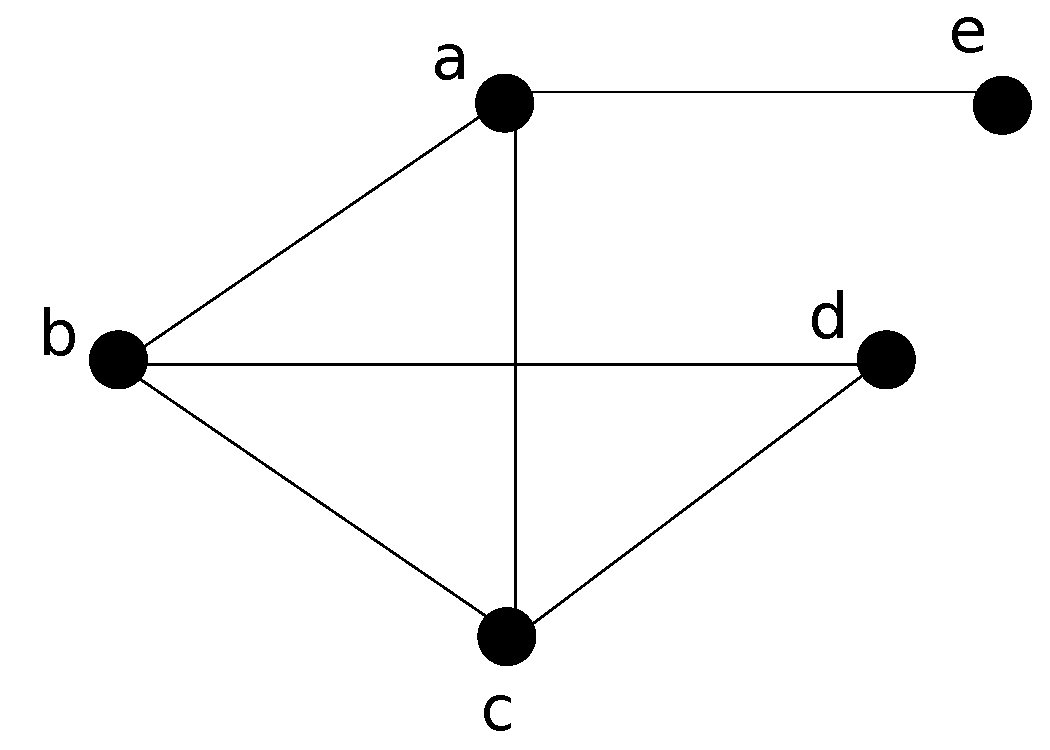
\includegraphics[width=.3\columnwidth]{connection}
		\caption{Social layer of graph $ G $}
		\label{fig:meet}
		\end{wrapfigure}  meeting point $ o_{1} $ to each member where  Figure \ref{fig:meet} represents social connection between these members. Let assume $ n'=3,c=1, V_I=\{a,b,e\}, V_R=\{c,d\} ,d_{m}=15, \alpha=.33, \beta=.33, \gamma =.33,|V|=5$. We have
		already got a result group where $ f_{c}=4 , d_{c} =35 $. But we
		are justifying whether including any vertex from $ V_R $ to  
		$V_I $ gives any better group. From R-tree indexing vertex $ d  $ is picked from $ V_R $. From Eq. \eqref{eq:terminate}, $ d_d^\uparrow=13.67 $. Now we have found that $ d(d,o1)=13<=d_d^\uparrow $ and $ f(d,V_I \cup \{d\}) =1 >=1 $. So according to Lemma \ref{lm:distance}, $ V_I \cup \{d\} $ is a better scored group than $ V_I $.

		
		\subsection{Terminating condition based on distance upper bound:}
		
		
		Lemma \ref{lm:distance} assures whether any member in $ V_R $ can be considered to be added in $ V_I $. But this does not help us to decide whether we can terminate our search for current $ V_R $. To terminate our search, we must assure that every member in $ V_R $ fails to generate any other better group. For simplicity we may assume that  new considered vertex $ v, v \in V_R $ is connected to every vertex of $ V_I $ which would give us distance upper bound for any member in $ V_R $. Let assume putting $ f_n=2*|V_I| $ in Eq. \eqref{eq:terminate} gives $ d^\uparrow=d_e $.
		
		
			\begin{equation}
			\label{eq:terminateDistance}
			\begin{split}
					\frac{d_m*(|V_I|+1)}{\beta}\Bigg(\frac{\alpha}{|V_I|*(|V_I|+1)}\bigg(2*|V_I|-
					\\
					\frac{2f_c}{(|V_I|-1)}
					\bigg)+
					\frac{\gamma}{|V|}\Bigg)+
					\frac{d_c}{|V_I|} >   d^\uparrow
			\end{split}		
			\end{equation}
			Here $ d^\uparrow $ is upper limit for $ d_{e} $.
			While retrieving vertex from $ V_R $, we take that vertex which is in minimum spatial distant from meeting point $ o' $. If $ v, v \in V_R $ is selected and $ d(v,o') > d^\uparrow$ current $ V_R $ can't produce any better scored group.
			
			
		
		\begin{Lemma}
			\label{lm:distanceUpper}
			If $ |V_I|>=n' , d(v,o')>d^\uparrow$ , $ v \in V_R $, the first retrieved vertex from $ V_R $ , $ V_R $ can never produce any better group.
		\end{Lemma}
		
		\begin{proof}
		 Since $ v $ is the first retrieved vertex from 
				$ V_R $ according to R-tree indexing, it is in minimum distant from meeting point $ o' $ than other vertices of $ V_R $. In this case,  $ d(v,o')>d^\uparrow $. So it is sure that no other vertices including $ v $ can be taken. 
		\end{proof}
		
		
						
				
		{Explanation:} Table ~\ref{tab:table4} shows distance from meeting point $ o_{2} $ to each member where Figure \ref{fig:meet} represents social connection between these members. Let assume $ n'=3,c=1, V_I=\{a,b,c\}, V_R=\{d,e\} ,d_{m}=15, \alpha=.33, \beta=.33, \gamma =.33,|V|=5$. We have already got a result group where $ f_{c}=6 , d_{c} =4 $. But we are justifying whether including any vertex from $ V_R $ to $ V_I $ gives any better group. From R-tree indexing vertex $ d  $ is picked from $ V_R $. Here $ d $ is closer to $ o_{2} $ than any other vertices of $ V_R $. From Eq. \eqref{eq:terminateDistance}, $ d^\uparrow=13.33 $. Now we have found that $ d(d,o1)=14 > d^\uparrow $ . So according to Lemma \ref{lm:distanceUpper}, further exploration of $ V_R $ will never produce any better group. So we can terminate our exploration for current meeting point.
		
		
		\subsection{Lower bound on Social Connectivity:}
		 Let assume, $ v $ is next retrieved member from $ V_R $ and $ v $ fails Lemma \ref{lm:distance} for $ d(v,o')>d_v^\uparrow $. But in our assumption we have taken $ f_{n}=2*c $ which is the lowest possible value for $ f_{n} $. If we still want to include $ v  $ in $ V_I $, it must satisfy good social connectivity to overcome considerably bad spatial distance and thus ensuring better score . 	 
		 
			\[
			\begin{aligned}
			\begin{split}
			&\frac{\alpha}{|V_I|*(|V_I|+1)}\bigg(f_n-\frac{2f_c}{(|V_I|-1)}
							\bigg)+
					\\
					& \frac{\gamma}{|V|}+
					\frac{\beta}{d_m*(|V_I|+1)}\bigg(\frac{d_c}{|V_I|}-d_e\bigg) > 0
			\\
			\Rightarrow
			&	\frac{\alpha}{|V_I|*(|V_I|+1)}\bigg(f_n-\frac{2f_c}{(|V_I|-1)}
									\bigg)
			\\
			&>
			\frac{\beta}{d_m*(|V_I|+1)}\bigg(d_e-\frac{d_c}{|V_I|}\bigg)-\frac{\gamma}{|V|}  	
			\\
			\Rightarrow
			&	f_n-\frac{2f_c}{(|V_I|-1)} >
			\frac{|V_I|*(|V_I|+1)}{\alpha}*
			\\
			&\Bigg(\frac{\beta}{d_m*(|V_I|+1)}\bigg(d_e-\frac{d_c}{|V_I|}\bigg)-\frac{\gamma}{|V|}\Bigg)
			\end{split}
			\end{aligned}
			\]
		
			
			
			
		 Putting $  d(v,o')=d_{e} $ in the above equation , we get  $ f^\downarrow = f_{n} $ which is   lower limit of social connectivity.	
			\begin{equation}
			\label{eq:lowerSocial} 
			\begin{aligned}
			\begin{split}
				f^\downarrow >
					\frac{|V_I|*(|V_I|+1)}{\alpha}
					\Bigg(\frac{\beta}{d_m*(|V_I|+1)}*
					\\
					\bigg(d(v,o')-\frac{d_c}{|V_I|}\bigg)-\frac{\gamma}{|V|}\Bigg)+\frac{2f_c}{(|V_I|-1)}
			\end{split}
			\end{aligned}
			\end{equation}
				 
	
		 
		 \begin{Lemma}
		 	\label{lm:spatial}
		 	If $ |V_I|>=n'$ and $ 2*f(v,V_I \cup \{v\}) >=f^\downarrow $ , $ V_I \cup \{v\} $ guarantees a better scored group than current $ V_I $. 
		 \end{Lemma}
		 \begin{proof}
		 The definition itself prove this Lemma because $ f^\downarrow $ is found from Eq.\eqref{eq:lowerSocial} and if   $ 2*f(v,V_I \cup \{v\}) >=f^\downarrow $, ~\ref{eq:familiarityLowerBound} or ~\ref{eq:familiarityUpperBound} is satisfied which guarantees better scored group as  $ V_I \cup \{v\} $. 
		 \end{proof}
		 
		
		Explanation: In example of Lemma \ref{lm:distance}, if $ d $ has distance of 14 from meeting point $ o_{1} $ then $ d(d,o1)> d^\uparrow $ ($ d^\uparrow=13.67 $ from Eq. \eqref{eq:terminate}). So $ d $ is not included into $ V_I $ for not satisfying Lemma \ref{lm:distance}. Now from Eq. \eqref{eq:lowerSocial}, $ f^\downarrow =2.067$ and $ 2*f(d,V_I \cup \{d\})= 2*1=2 < f^\downarrow $. So according to Lemma \ref{lm:spatial}  $ d  $ is still not taken. But vertex    $ c $ also has distance 14. So putting it's distance in Eq. \eqref{eq:lowerSocial} also produces $ f^\downarrow =2.067$ and $ 2*f(c,V_I \cup \{c\})= 2*2=4 >= f^\downarrow $. So according to Lemma \ref{lm:spatial} , $ c $ is included in $ V_I $ for $ V_I \cup \{c\} $ being proved to be better scored group than $ V_I $.
			
	 	
		
		
		
		\section{Pruning strategy for next meeting points}
		We can develop some pruning strategy when we have already found relevant group. Let assume that $ f_o, n_o, d_o $ be the $ k_{th} $ group's total social connectivity, number of member in that group and total spatial distance from corresponding meeting point respectively. While exploring group for current meeting point $ o_{c} $, let assume that $ f_{c}, d_{c} $ be total social connectivity currently explored in $ V_I $  and total spatial distance of  all members of $ V_I $ from meeting point $ o_{c} $ respectively. we will explore more for $ o_{c} $ if we are guaranteed to get better group in future. For better group the following condition has to be satisfied. 
		
		
		\begin{equation}
		\label{eq:second_terminate}
		\begin{split}
		\alpha \left(\frac{f_{c}+f_n}{n'*(n'-1)}-\frac{f_o}{n_o*(n_o-1)}\right)+
		\frac{(n'-|V_I|)*\gamma}{|V|}
		\\		 	
		+\frac{\beta}{d_{m}}\left(\frac{d_o}{n_o} -\frac{d_{c}+d_n}{n'}\right)	> 0 	
		\end{split}
		\end{equation}
		
		The idea of Eq. \eqref{eq:second_terminate} is derived from Eq. ~\eqref{eq:better}.
		In Eq. \eqref{eq:second_terminate} we have two unknown variable, $ f_n $ and $ d_n $. To get a upper limit of $ d_{e} $ like Eq. \eqref{eq:terminateDistance} we may assume that the vertices that will be included into $ V_I $ from $ V_R $ for current meeting point $ o_{c} $ will be connected with every vertex from $ V_I $. This results in an upper bound for $ d_{e} $. For this assumption-
		\begin{equation*}
		\begin{split}
				\begin{aligned}
				s'_{new}&=|V_I|+|V_I|+1+|V_I|+2+....+(|V_I|+n'-|V_I|-1) 
				\\
				 &= \frac{(n'-|V_I|)*(n'+|V_I|-1)}{2} 		
				\end{aligned}
		\end{split}
		\end{equation*}
	
		Putting $ f_n=2*s'_{new} $ in Eq. \eqref{eq:second_terminate} gives  upper limit for $ d_{e} $ which is denoted as $ d^\uparrow $.
		\begin{equation}
		\label{eq:nextTerminate}
		\begin{split}
		n'\Bigg(\frac{d_{m}}{\beta}\bigg(\alpha \left(\frac{f_{c}+2*s'_{new}}{n'*(n'-1)}-\frac{f_o}{n_o*(n_o-1)}\right)+
		\\
		\frac{(n'-|V_I|)*\gamma}{|V|}\bigg)-\frac{d_o}{n_o}\Bigg)+d_{c}=d^\uparrow		
		\end{split}
		\end{equation}
		Here, $ d^\uparrow $ is distance upper bound for  cumulative distance  	of next to be explored vertices from $ V_R $. If $ d_{min} $ is the immediate selected vertex from $ V_R $ (which is minimum for other vertices of $ V_R $) , for assurance of better group the following condition must be held.
		\[
		d^\uparrow \geq d_{min}*(n'-|V_I|) 
		\]
		
		\begin{Lemma}
			\label{lm:final}
			For any meeting point $ o_{c} $, if $ d^\uparrow < d_{min}*(n'-|V_I|) $ , then current exploration for $ o_{c} $ can never produce any better scored group.
		\end{Lemma}
		
		\begin{proof}
		 If $ d^\uparrow < d_{min}*(n'-|V_I|) $, then current exploration results in a group which does not satisfy Eq. ~\ref{eq:familiarityLowerBound} or ~\ref{eq:familiarityUpperBound} . This group might satisfy minimum acquaintance constraint or produce better social connectivity but lags in $ score_{spatial} $. So search for $ o_{c} $ must be terminated.
		\end{proof}
		
		
		Explanation: Let's assume our search begins with meeting point $ o_{2} $ and we have found a resultant group described in example of Lemma \ref{lm:distanceUpper}. For simplicity we may assume that this group is the $ k_{th} $ group of list L. Here selected vertex set=$ \{a,b,c\} $, $ d_o=4,f_o=6,n_o=3 $. Now while starting searching for meeting point $ o_{1} $ we have $ d_{c}=0,f_{c}=0,f_{n}=3, |V_I|=0 $. According to Eq. \eqref{eq:nextTerminate}, $ d^\uparrow=23 $.  Now vertex $ a  $ is selected from $ V_R $ at first. So $ d_{min}=d(a,o1)=10 $ and $ 23 < 10*(3-0)=30 $. So according to Lemma \ref{lm:final} further exploration for meeting point $ o_{1} $ can never produce any better group than the first group. So search terminates for $ o_{1} $. 
		
		
		
		
		
		
		
		
		\begin{algorithm*}
		%\begin{multicols}{2}
		
		\DontPrintSemicolon
		
		\SetAlgoLined
		
		%\KwResult{Write here the result}
		
		\SetKwInOut{Input}{Input}\SetKwInOut{Output}{Output}
		\SetKwFunction{FindGroup}{FindGroup}
		\Input{Graph $ G=(V,E) $, user location $ l_v  $ for each $ v \in V $,  minimum number of member in a group $ n' $, activity location set $ O $, minimum acquaintance constraint $ c $, spatial radius $ d_{m} $. The user location $ l_v,\forall v \in V $ are indexed by R-tree. }
		
		\Output{A priority queue list $ L  $ of $k$ tuples in descending order of socio spatial group score. Each tuple contains a group $ G' $, socio spatial group score and corresponding meeting point $ o' $.}
		
		\BlankLine
		\ForEach{meeting point $  o_i \in O $}{
		Initialize $ V_I = \varnothing , \theta = c$\;
		Employ R-tree Range Query on $ o_i $ to find the vertices  within distance $ d_{m} $ as $ V_R $\;
		Discard unqualified vertices from $ V_R $ which does not satisfy familiarity constraint in $ V_R $\;
		\FindGroup{$V_I,V_R,o_i$}\;
		
		}
		
		
		\SetKwProg{myproc}{Procedure}{}{}
		\myproc{\FindGroup{$inV_I,inV_R,o_i$}}{
		$ V_I\leftarrow in V_I, V_R\leftarrow in V_R $\;
		\While{$ (|V_I|+|V_R| \geq n' ) $ and $  |V_R| > 0 $}{
		$ d_{min}=\infty $	\;
		\uIf{there is any unvisited vertex in $ V_R $}{
		Employ R-tree distance browsing to extract from $ V_R $ the next unvisited vertex $ u $ which has the minimum spatial distance to $ o_i $\;
		mark $ u $ as visited\;
		$ d_{min}\leftarrow d(u,o_i) $\;
		}
		\Else{
			return\;
		}
		\uIf{$ |V_I|<n' $ and $ u $ satisfies Eq. ~\eqref{eq:familiarityLowerBound} or ~\eqref{eq:familiarityUpperBound}}{
			
				\uIf{ Lemma \ref{lm:final} is satisfied }{
					return \;
				}
				$ V_I \leftarrow V_I \cup \{u\}$\;
				$ V_R \leftarrow V_R - \{u\} $\;
				\uIf{$ \delta(V_I) <c$}{
					$ V_I \leftarrow V_I - \{u\}$\;
					
					continue \;
				}		
				Update $ L $ in descending order of score with new result group $ V_I $ \;
				
				\FindGroup{$V_I,V_R,o_i$}\;
				$ V_I \leftarrow V_I - \{u\}$\;
				
			
			
		}
		\Else{
			\uIf{$ f(u, V_I)  >=c$}{
				\uIf{ $ L $ is not full}{
					$ V_I \leftarrow V_I \cup \{u\}$\;
					$ V_R \leftarrow V_R - \{u\} $\;
					Update $ L $ in descending order of score with new result group $ V_I $ \;
					
					\FindGroup{$V_I,V_R,o_i$}\;
					$ V_I \leftarrow V_I - \{u\}$\;
					continue\;	
				}
				\uIf{$ L $ was updated with $ V_I $ in previous call}{
					$ V_I \leftarrow V_I \cup \{u\}$\;
					$ V_R \leftarrow V_R - \{u\} $\;
					Update $ L $ in descending order of score with new result group $ V_I $ \;
					
					\FindGroup{$V_I,V_R,o_i$}\;
					$ V_I \leftarrow V_I - \{u\}$\;
				}
				\Else{
					\uIf{ Lemma \ref{lm:distanceUpper} is satisfied }{
						return \;
					}
					\uIf{ Lemma \ref{lm:distance} or Lemma \ref{lm:spatial} is satisfied}{
						$ V_I \leftarrow V_I \cup \{u\}$\;
						$ V_R \leftarrow V_R - \{u\} $\;
						Update $ L $ in descending order of score with new result group $ V_I $ \;
						
						\FindGroup{$V_I,V_R,o_i$}\;
						$ V_I \leftarrow V_I - \{u\}$\;
							
					}
				}
				
			}
			
		}
		
		
	
		
		}
		
		}
		
		
		\caption{SSTk}
		%\end{multicols}
		\end{algorithm*}
		
		
		
		
		
		
		
		%\nocite{*}
		\bibliographystyle{abbrv}
		\bibliography{draft11}  % vldb_sample.bib is the name of the 
\end{document}